\section{Introduction}

Some practical sections in this manual is based on the writing of
\cite{12gr730}. Going further to describe the use cases when using
AAUSHIP in a formation control setup will be described here.

The use case considered here is that of \ac{ASV} Formation Control for
Surveying Purposes. This task is about using the \ac{ASV} to scan an
area using a ``lawnmower''-pattern. This pattern is of course not a
very definite pattern, but it basically means that the mowing machine
or formation in this case will move across all the area in some structured way.

\section{Description} The AAUSHIP consists of an approximately 1 meter
long vacuum formed hull made of ABS plastic, which contains twin
propellers. Additions on some AAUSHIPs include tunneltrusters for
those that want to include this option.

\begin{figure}[htbp]
	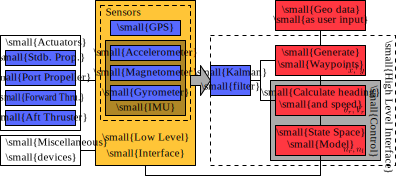
\includegraphics[width=\textwidth]{fig/vessel-block-overview}
	\caption{Overview of the control layout and its interfaces for a
		single AAUSHIP.
		Modified version of graphic from \citep{12gr730}.}
	\label{fig:vessel-block-overview}
\end{figure}

\section{Important things}
When doing formation control it is important to figure out what one
want to achieve, and depending on the strategy and the formation type
some things are to be considered as requirements regarding how the
formation should work. We are considering lawnmower patterns in this
discussion. In this work two ships are considered for simplicity, but
it should be extensible to n-number of ships.

When starting the mission, the ships may start at positions that
is not in the desired formation, it is important that the ships are in
formation when they start tracking the desired track. Therefor some
attention must be given on how to make the ships initialize this
formation. An approach is to make the ships sail individually to the
starting positions with a speed that makes them hit their respectively starting points at
the same time. If one reaches its start point much earlier
than the other it must stop, which is not wanted because it then can
drift out of position again. This basically means that there is a
tracking phase and an initialization phase. The start heading should of
course align with the path at that point.

Another issue to be considered is to ensure that no ship at
any point in time reaches a minimum speed that is necessary for the
ship to not drift out of formation. This could be a problem in corners
of the formation if a stiff construction, where the inner most ship
has to move slower, to accommodate the shorter distance on an inner
circle arc.

Faults like blackout on a ship could also be considered in the control
design. I.e. what happens with the formation when one ship faults in a
blackout. Should the rest of the formation stop, should the formation
still follow this drifting ship or should the mission simply terminate
when it is discovered that a ship has blackout.

In the initialization phase it is also relevant to consider how the
ships should avoid each other if they are on the wrong side of each
other.

\begin{figure}[htbp]
	\centering
	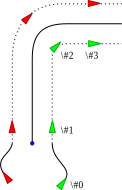
\includegraphics[width=0.8\textwidth]{fig/cornoring}
	\caption{Two ships initializing and following the path offset
		equally on each side, ships are constrained to sailing parallel
		and heading the same as path when projected onto the path. Blue
	dot is start of path. Fully drawn splines is initializing phase.}
	\label{fig:cornoring}
\end{figure}

On figure~\vref{fig:cornoring} is a simple path following performed
with two ships in a stiff formation with an equal distance from the
path. It illustrates four steps, in step \#0 the ships initializes a
random position near the start of the path. At \#1 it is tracking the
path in formation, whilst still in formation. At \#2, the green
(right) ship is in a tight inner curve where it is important to
consider design of the path such that the capabilities of the ship is not
exceeded to stay in formation. At \#3 it is back to straight line path
following in formation.


\subsubsection{Degree of Actuation}
The degree of actuation is a matter that sets some limitations on how
the path following can be made, and thus the methods available to
control the ships.

AAUSHIP is a ship, which means that is is not fully actuated in the
whole 3D space, but this is not needed since it is moving on a
surface. To be fully actuated it must be able to have controls for
surge, sway and yaw.

\todo{State if it is fully actuated in this sense}
